\chapter{Конструкторский раздел}
\label{cha:design}

В данном разделе будет произведена разработка конвейера умножения матриц по алгоритму Винограда.

\section{Функциональная модель}
На рисунке \ref{img:idef0} представлена функциональная модель IDEF0 уроня 1.
\begin{figure}
    \centering
    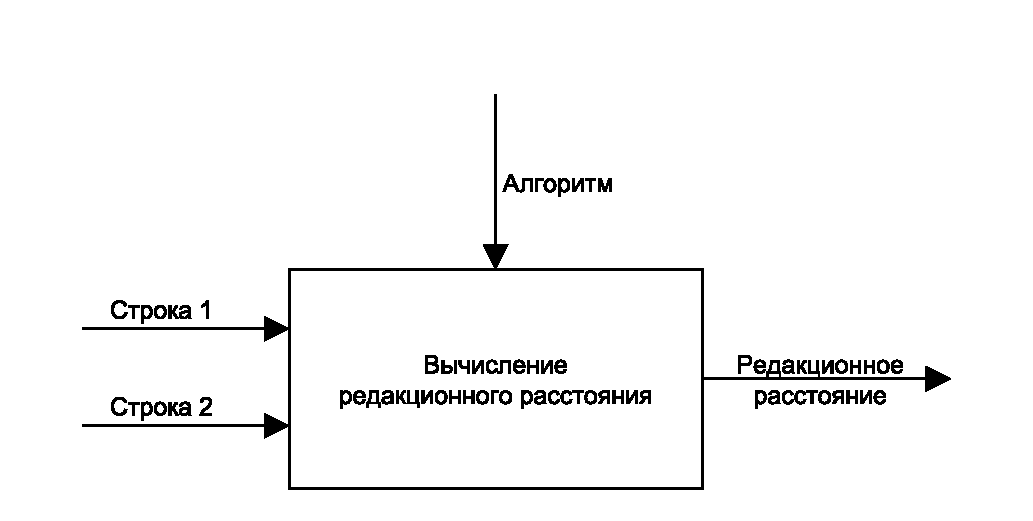
\includegraphics[scale=.7]{pdf/mainIdef0.pdf}
    \caption{функциональная модель IDEF0 уроня 1}
    \label{img:idef0}
\end{figure}

\section{Разработка алгоритмов}
Изобразим схемы алгоритма Винограда и конвейера умножения матриц по этому алгоритму.

\subsection{Алгоритм Винограда}

На риснуках \ref{img:windograd1}, \ref{img:windograd2} изображена схема алгоритма Винограда.
\begin{figure}[H]
    \centering
    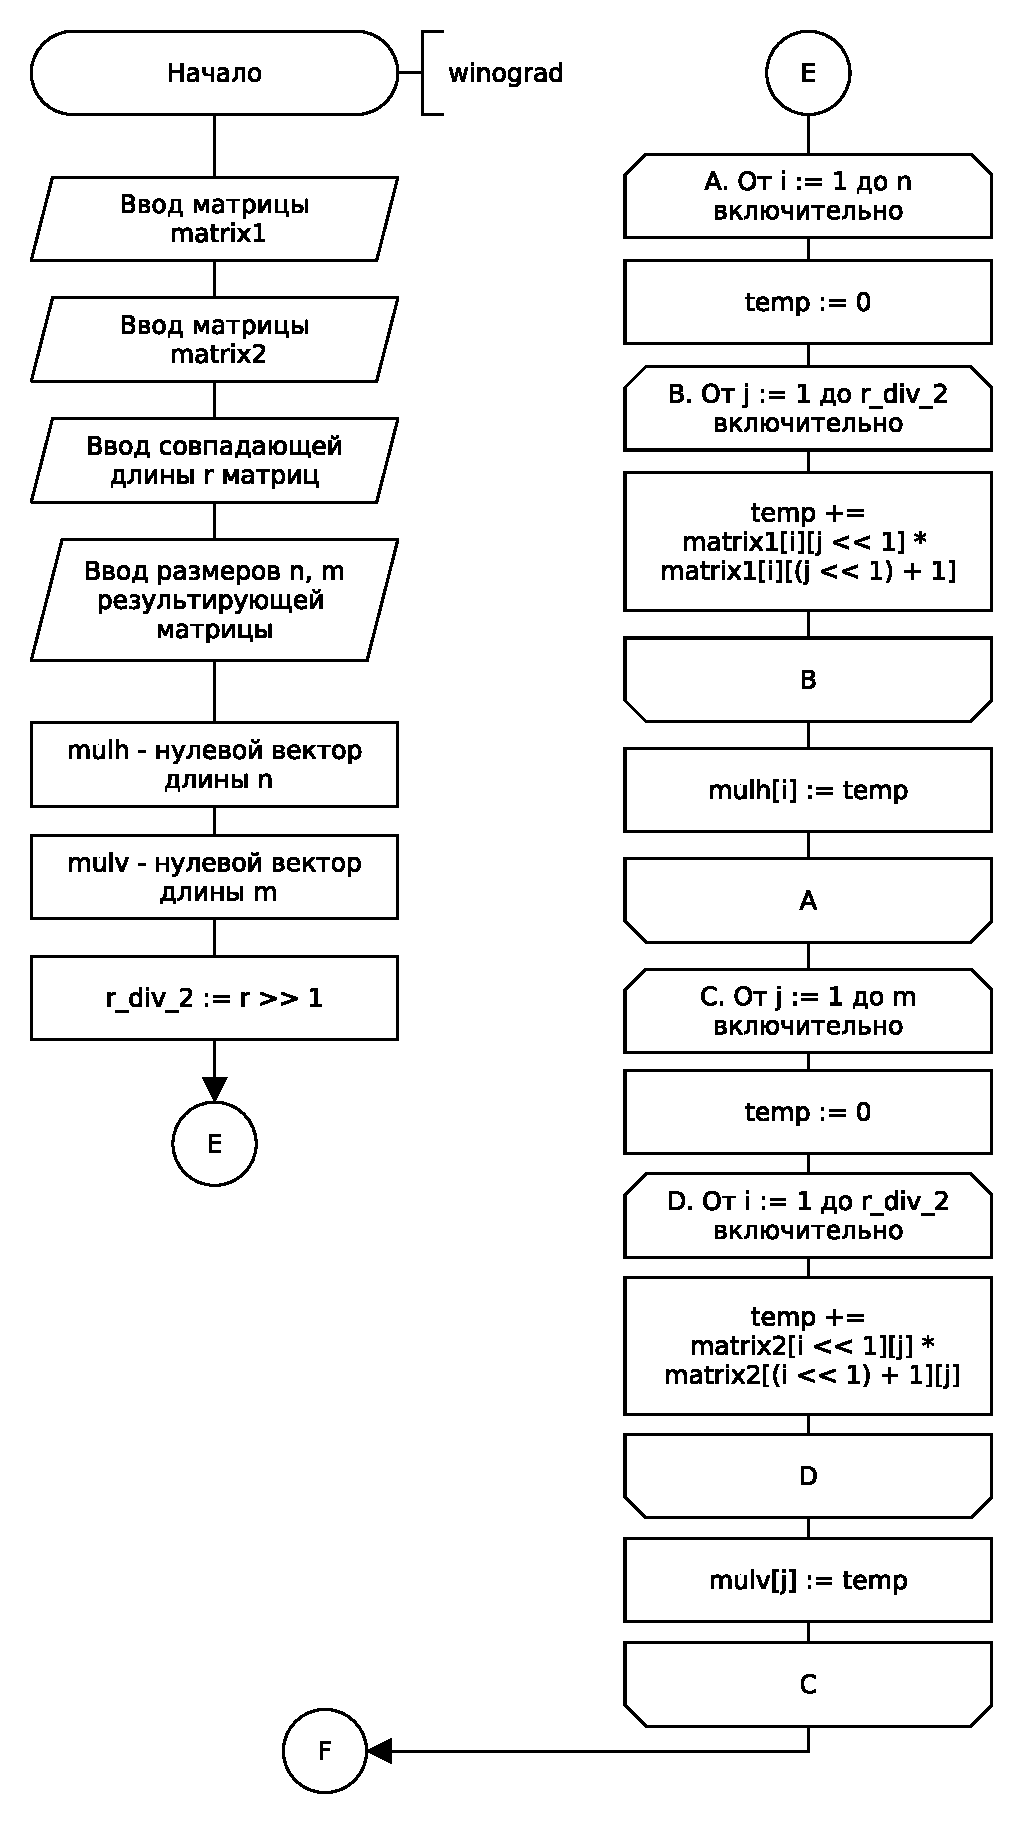
\includegraphics[scale=0.70]{pdf/owinograd-part1.pdf}
    \caption{Алгоритм Винограда, часть 1}
    \label{img:windograd1}
\end{figure}

\begin{figure}[H]
    \centering
    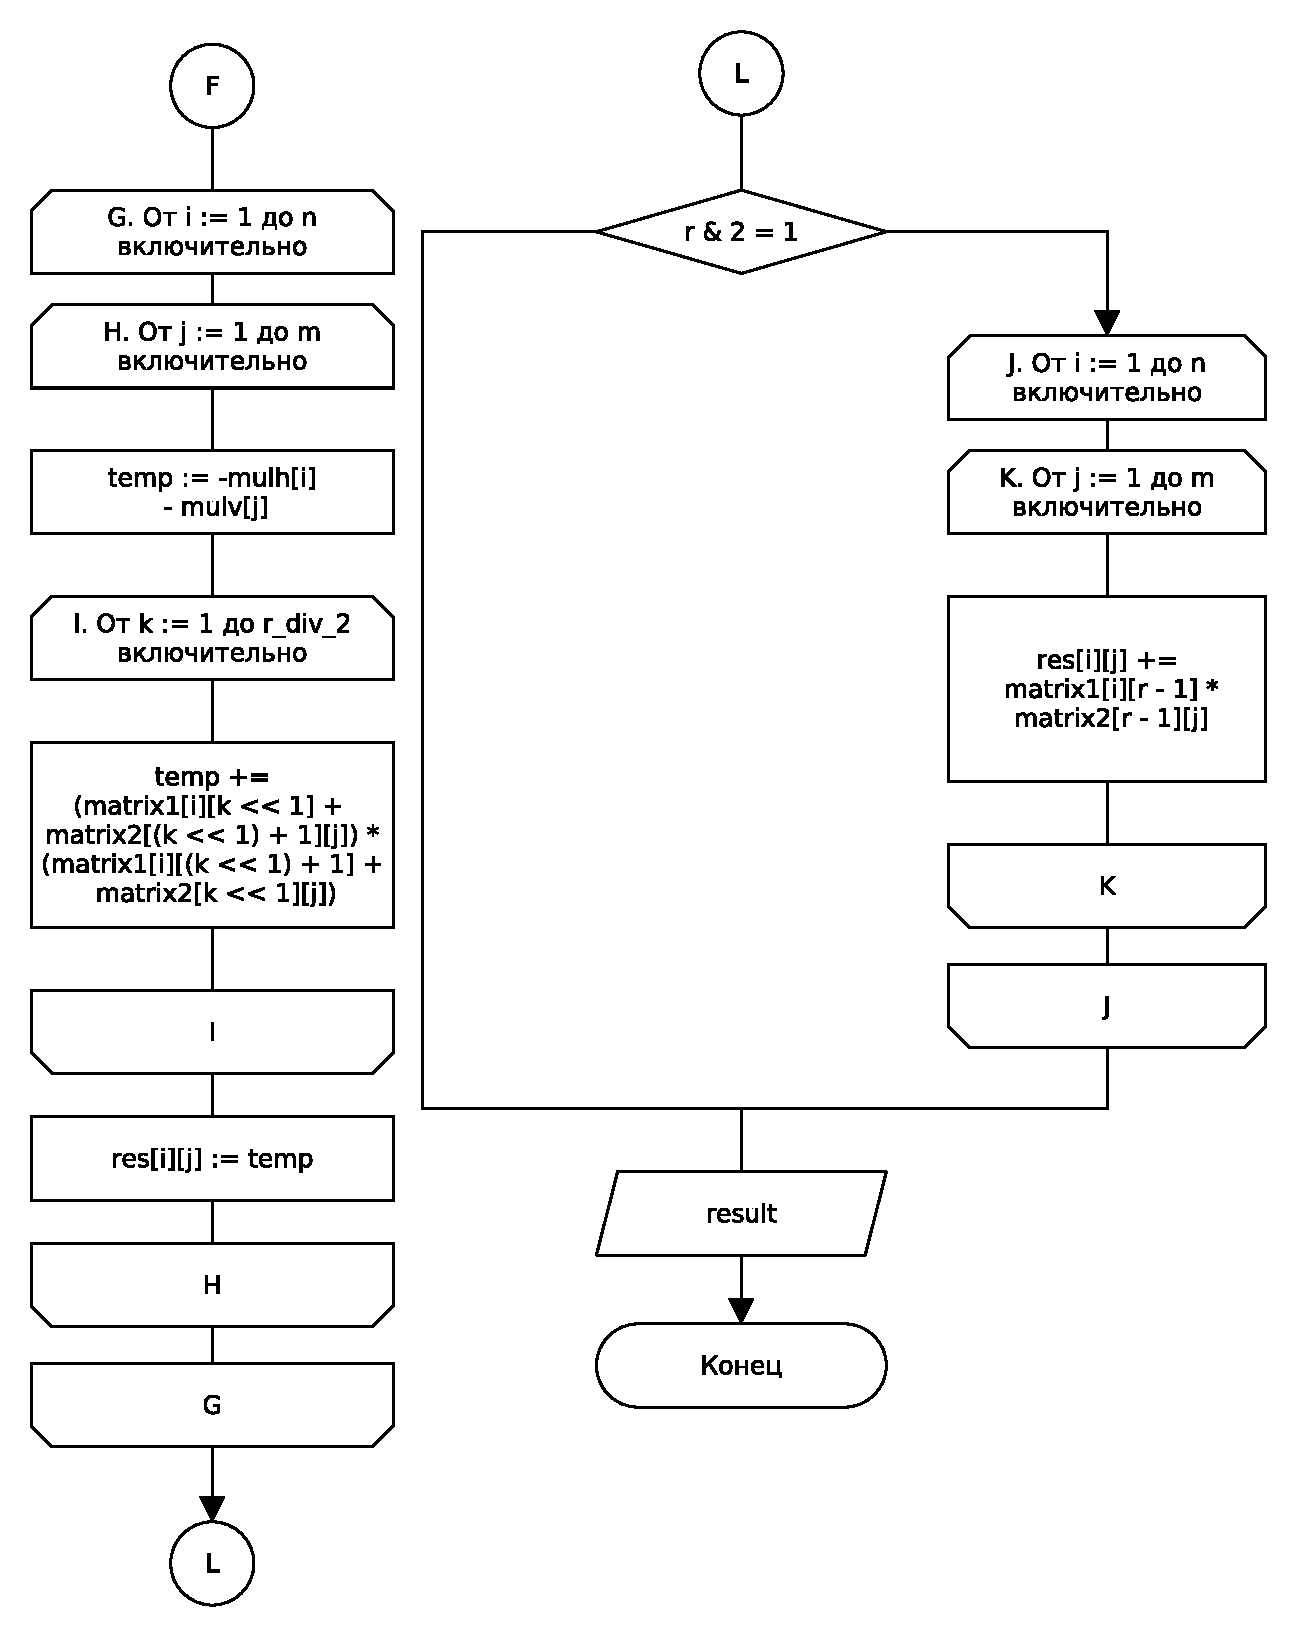
\includegraphics[scale=0.70]{pdf/owinograd-part2.pdf}
    \caption{Алгоритм Винограда, часть 2}
    \label{img:windograd2}
\end{figure}

\subsection{Конвейер}

Для того, чтобы распараллелить алгоритм Винограда по линиям конвейера выделим следующие этапы:
\begin{enumerate}
    \item ввод матриц, выделение необходимой для вычислений памяти;
    \item вычисление вектора mulh;
    \item вычисление вектора mulv;
    \item вычисление первой половины матрицы-произведения;
    \item вычисление второй половины матрицы-произведения;
    \item проверка чётности и вычисления оставшейся части матрицы.
\end{enumerate}

На рисунке \ref{img:cwindograd} приведена схема конвейера, вычисляющего произведение матриц по алгоритму Винограда.

\begin{figure}[H]
    \centering
    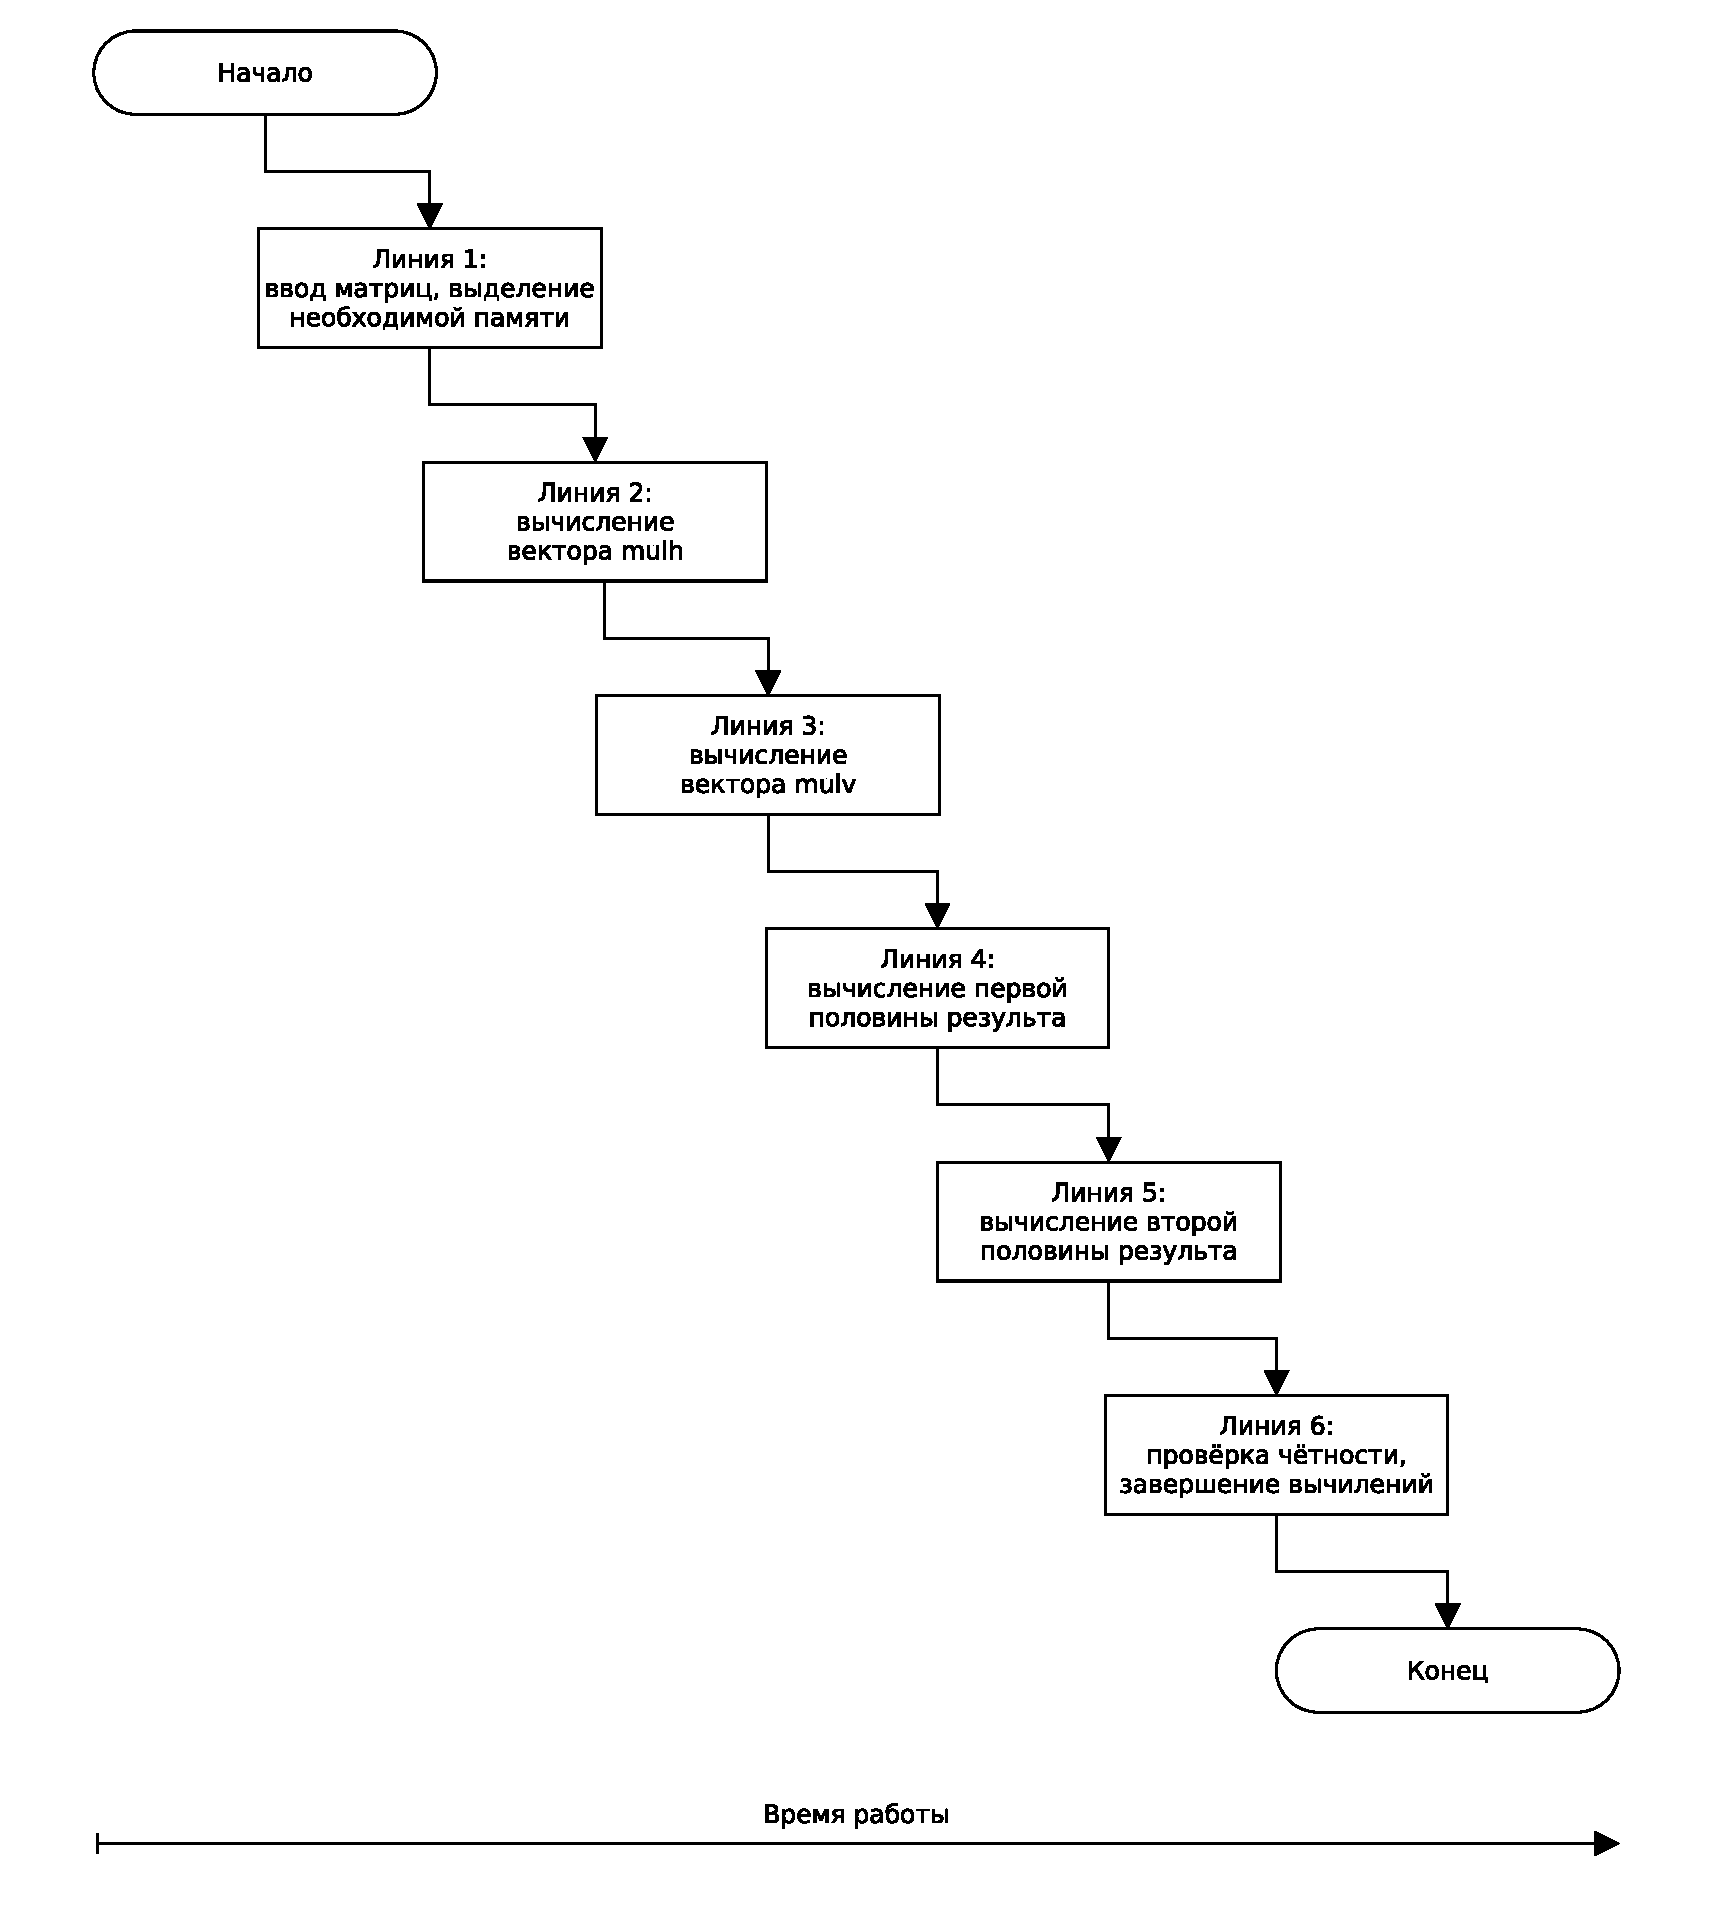
\includegraphics[scale=0.5]{pdf/cwinograd.pdf}
    \caption{Схема конвейера перемножения матриц по алгоритму Винограда}
    \label{img:cwindograd}
\end{figure}

\section{Вывод}
Благодаря тому, что вычисление каждого элемента матрицы произведения независимо от остальных, удалось разработать параллелизированный алгоритм Винограда.

